\subsection{1. Giao diện sản phẩm}
\indent\indent\textbf{Trang chủ:} Ứng dụng ICH Predictor được thiết kế tích hợp toàn bộ quy trình xử lý trên một trang duy nhất. Giao diện chính được minh hoạ tại \textbf{Hình} \ref{fig:TrangChu-1} và \textbf{Hình} \ref{fig:TrangChu-2}, bao gồm các nhóm chức năng chính: Quản lý tệp tin (Thêm tệp/Hoàn tất), Chọn mô hình và tiến hành dự đoán. Hệ thống hỗ trợ linh hoạt ba kịch bản dự đoán: đơn phương thức (chỉ ảnh), đa phương thức chỉ dùng hình ảnh và văn bản và đa phương thức toàn diện. Tương ứng với mỗi kịch bản, người dùng có thể lựa chọn các phiên bản mô hình đã được huấn luyện.
\begin{figure}[H]
    \centering
    \fbox{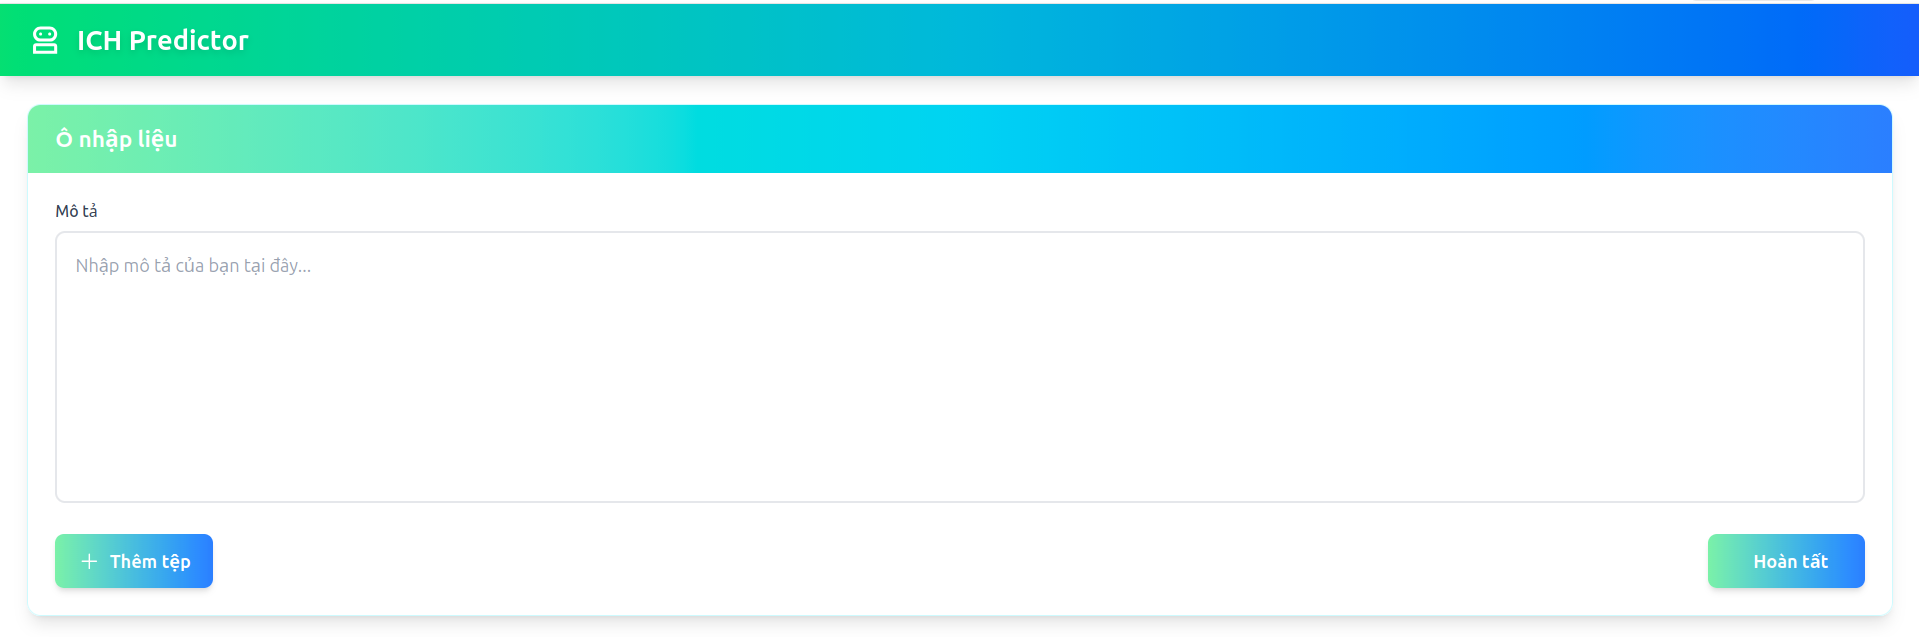
\includegraphics[width=0.9\linewidth]{images/part-02/chap-03/sec-01/TrangChu-1.png}}
    \vspace{0.1cm}
    \caption{Giao diện trang chủ -- Khu vực nhập liệu, thêm và hoàn tất tải tệp lên}
    \label{fig:TrangChu-1}
\end{figure}

\begin{figure}[H]
    \centering
    \fbox{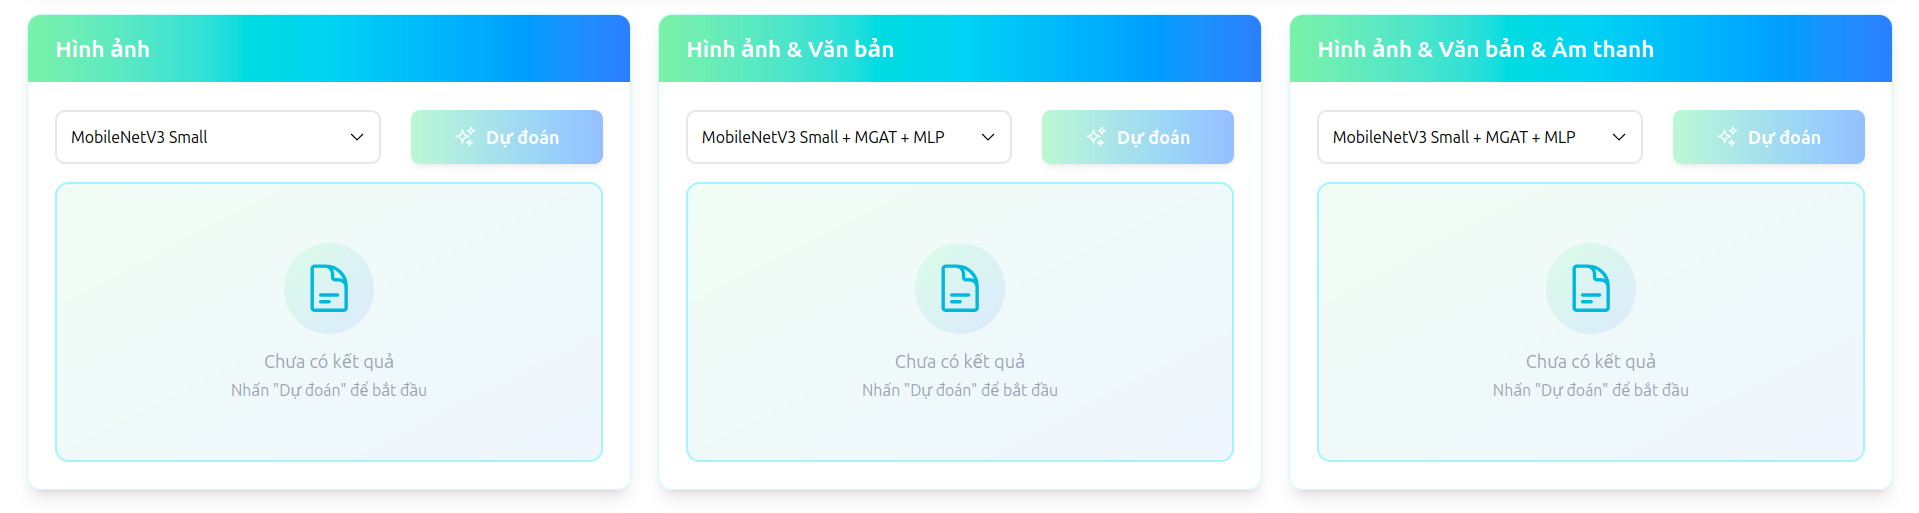
\includegraphics[width=0.9\linewidth]{images/part-02/chap-03/sec-01/TrangChu-2.png}}
    \vspace{0.1cm}
    \caption{Giao diện trang chủ -- Khu vực hiển thị kết quả}
    \label{fig:TrangChu-2}
\end{figure}

\newpage
\textbf{Quản lý tệp tin:} Khi người dùng tương tác với chức năng "Thêm tệp", hệ thống hiển thị một cửa sổ cho phép tải lên dữ liệu. Tại đây, các tệp tin được kiểm tra tự động để đảm bảo tuân thủ các ràng buộc về định dạng và kích thước đã đề ra.
\begin{figure}[H]
    \centering
    \fbox{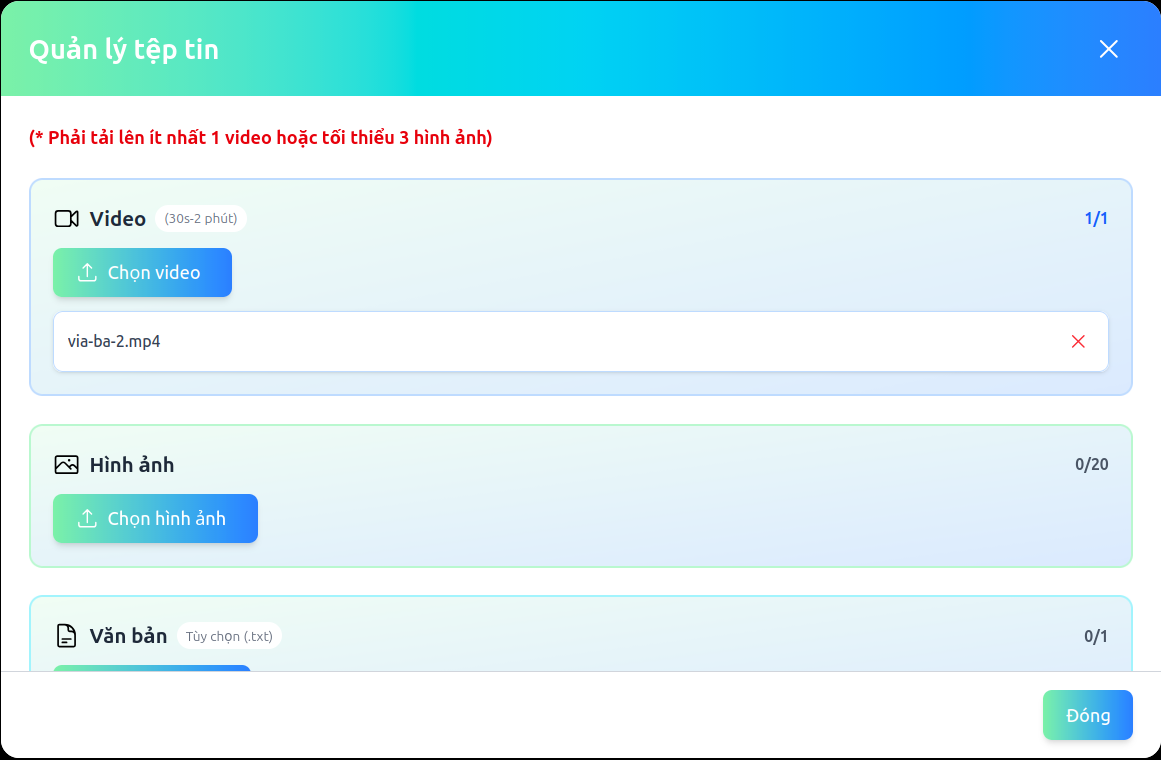
\includegraphics[width=0.9\linewidth]{images/part-02/chap-03/sec-01/ThemTep.png}}
    \vspace{0.1cm}
    \caption{Giao diện modal cho phép thêm tệp tin đa phương thức}
    \label{fig:ThemTep}
\end{figure}

\textbf{Hoàn tất tải lên:} Sau khi lựa chọn dữ liệu, người dùng xác nhận bằng nút "Hoàn tất". Lúc này, dữ liệu và nội dung mô tả được đẩy lên máy chủ để kích hoạt quy trình tiền xử lý (bao gồm phân tách video và trích xuất đặc trưng sơ bộ). Cơ chế này giúp tối ưu hóa thời gian phản hồi khi thực hiện lệnh dự đoán sau đó. Hình minh họa dưới đây thể hiện trạng thái khi dữ liệu đã được đồng bộ thành công lên máy chủ.
\begin{figure}[H]
    \centering
    \fbox{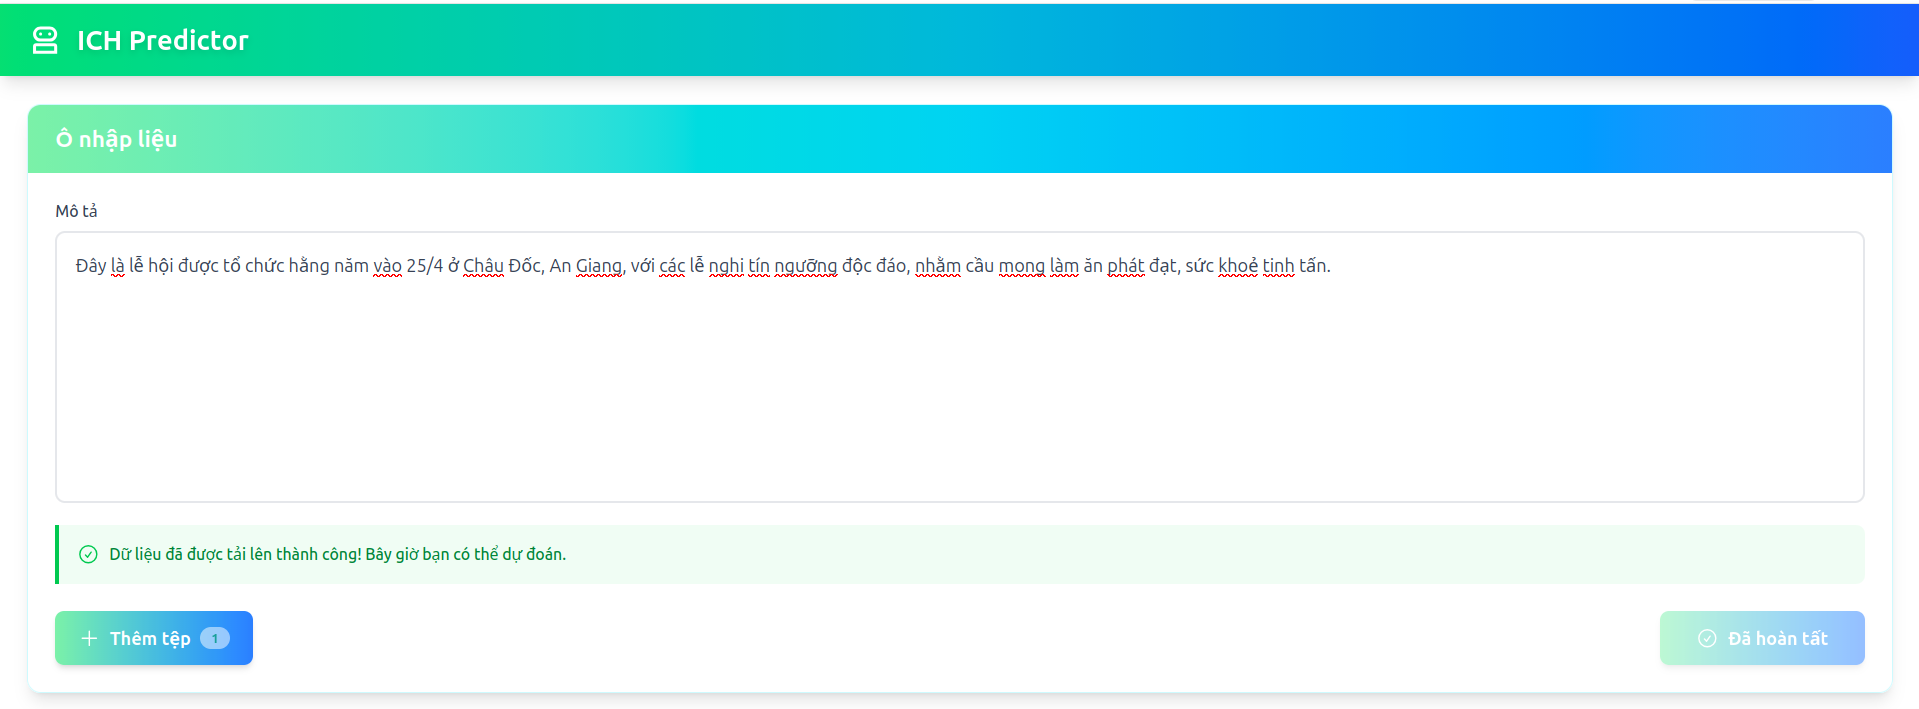
\includegraphics[width=0.9\linewidth]{images/part-02/chap-03/sec-01/UploadThanhCong.png}}
    \vspace{0.1cm}
    \caption{Giao diện hiển thị trạng thái tải tệp và nội dung mô tả thành công}
    \label{fig:UploadThanhCong}
\end{figure}

\newpage
\textbf{Kết quả dự đoán:} Người dùng lựa chọn kiến trúc mô hình mong muốn (ví dụ: MobileNetV3 Small) và kích hoạt quá trình dự đoán. Hệ thống sẽ trả về kết quả bao gồm nhãn chủ đề văn hóa dự đoán và chỉ số độ tin cậy tương ứng.
\begin{figure}[H]
    \centering
    \fbox{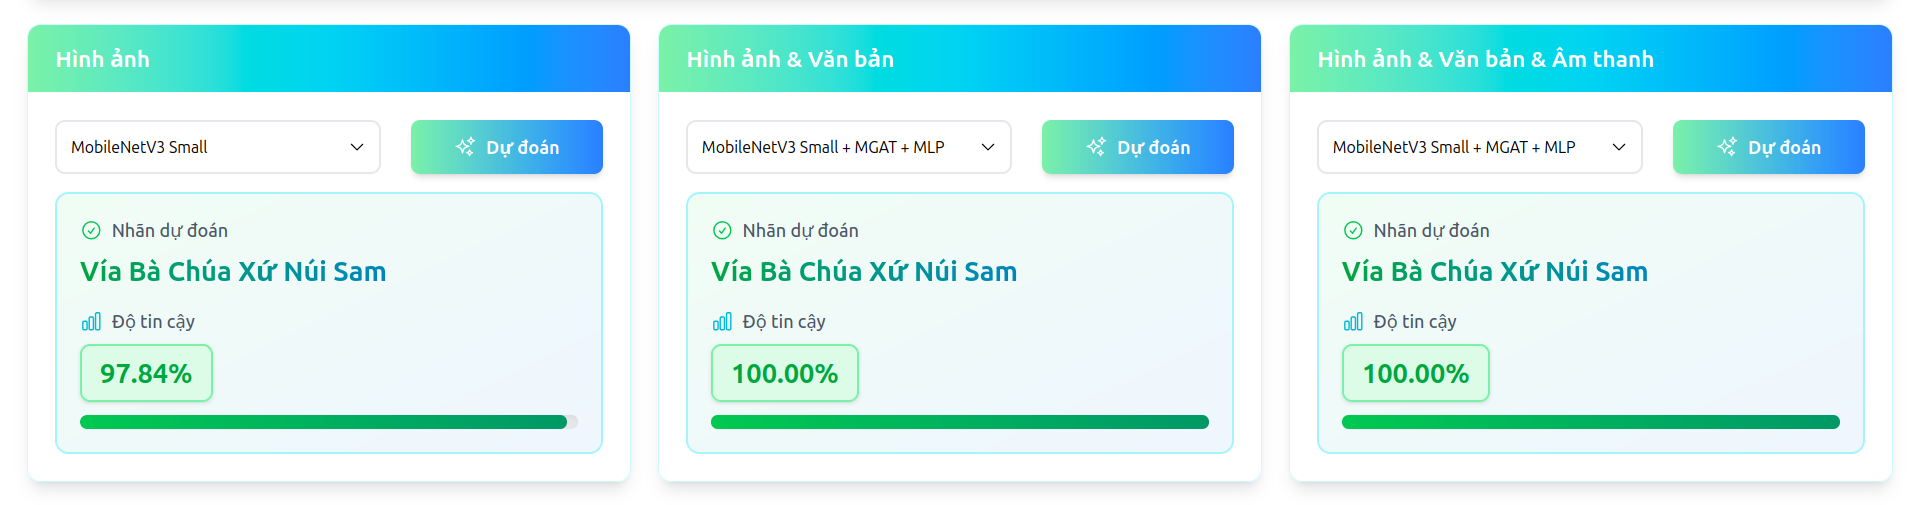
\includegraphics[width=0.9\linewidth]{images/part-02/chap-03/sec-01/KetQua.png}}
    \vspace{0.1cm}
    \caption{\centering Giao diện hiển thị kết quả dự đoán với mô hình backbone MobileNetV3 Small}
    \label{fig:KetQua}
\end{figure}

\textbf{Đồ thị:} Đối với các kịch bản dự đoán đa phương thức, khu vực kết quả cung cấp thêm công cụ trực quan hóa cấu trúc đồ thị. Giao diện này cho phép người dùng xem xét danh sách các nút (đỉnh) tham gia vào quá trình suy luận và hiển thị trực quan các kết nối giữa chúng.
\begin{figure}[H]
    \centering
    \fbox{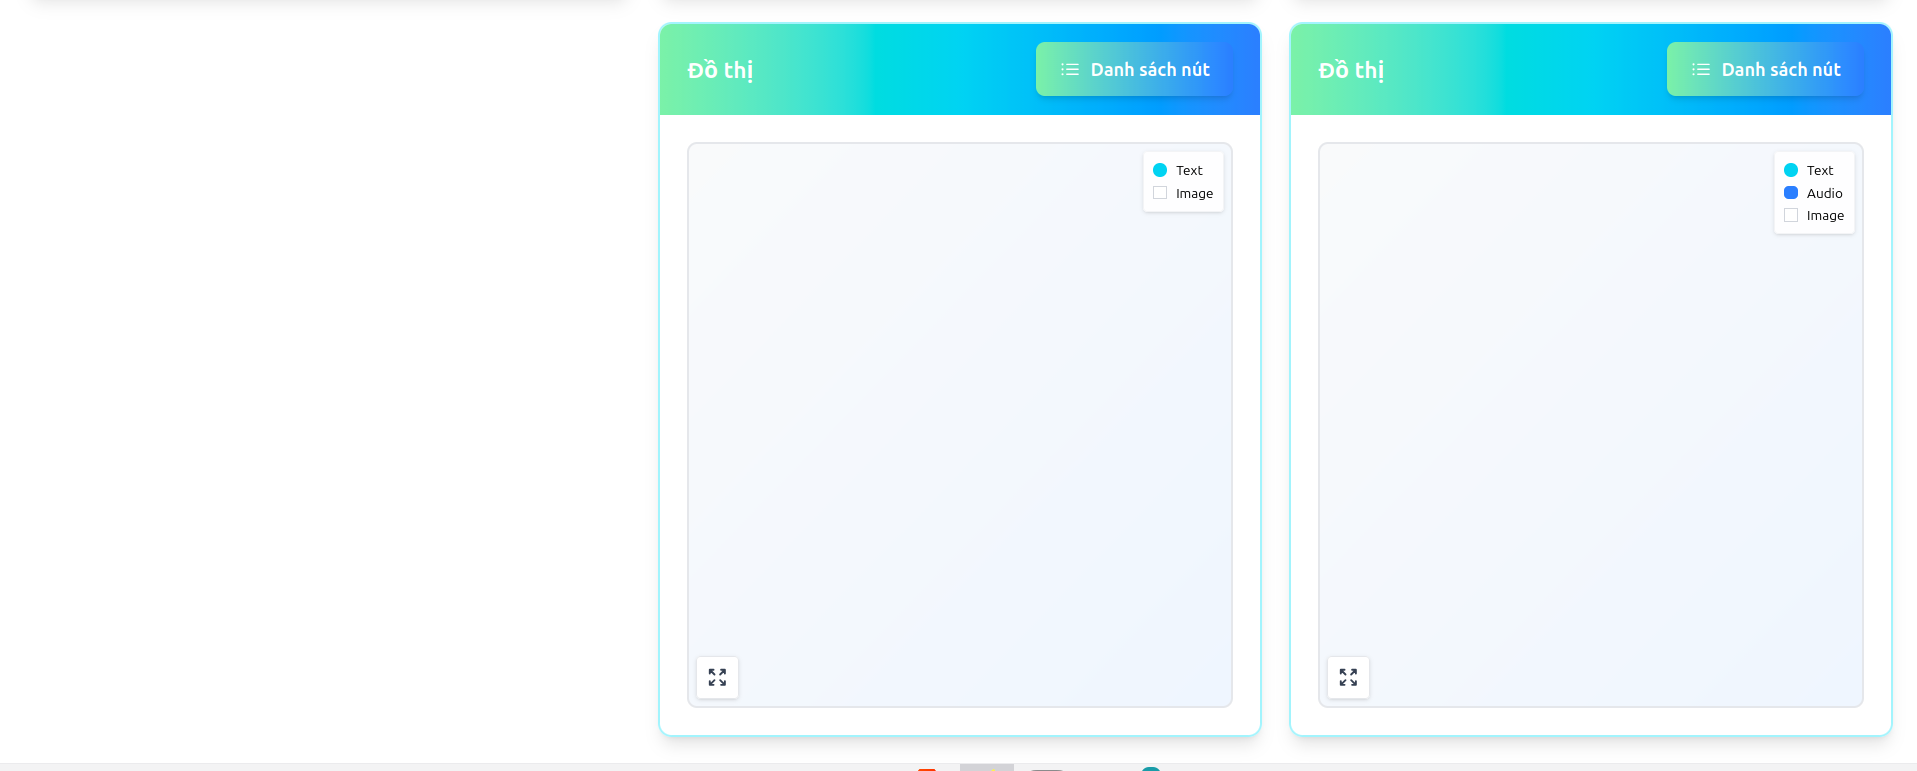
\includegraphics[width=0.9\linewidth]{images/part-02/chap-03/sec-01/DoThi.png}}
    \vspace{0.1cm}
    \caption{Giao diện công cụ trực quan hóa đồ thị cho mô hình MGAT + FastKAN/MLP}
    \label{fig:DoThi}
\end{figure}

\newpage
\textbf{Danh sách nút hình ảnh:} Khi bấm vào nút "Danh sách nút", người dùng có thể tùy chọn các nút hình ảnh cụ thể để hiển thị. Đồng thời, hệ thống cung cấp các bộ lọc để lọc các cạnh kết nối dựa trên ngưỡng trọng số (hiển thị top \% các cạnh có trọng số cao nhất), giúp giảm nhiễu khi quan sát.
\begin{figure}[H]
    \centering
    \fbox{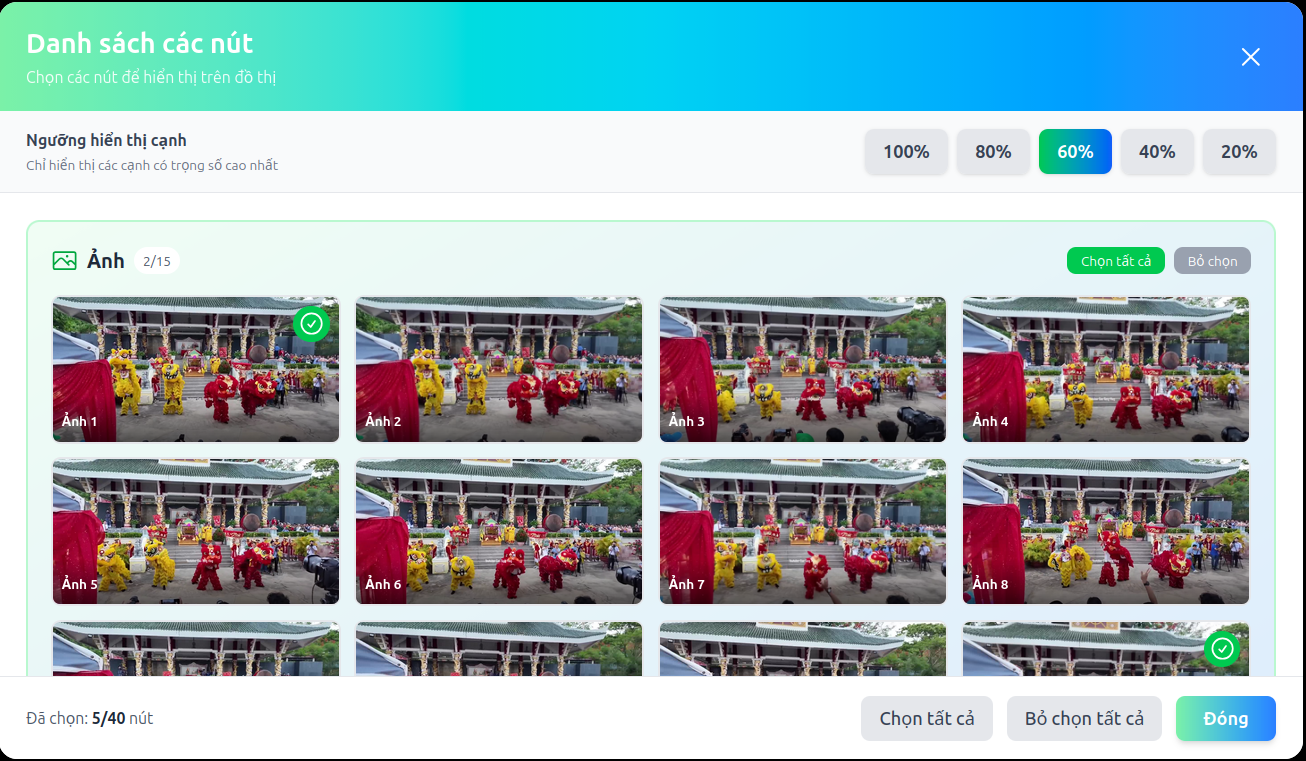
\includegraphics[width=0.9\linewidth]{images/part-02/chap-03/sec-01/DSNut-HinhAnh.png}}
    \vspace{0.1cm}
    \caption{Giao diện danh sách nút cho phương thức hình ảnh}
    \label{fig:DSNut-HinhAnh}
\end{figure}

\textbf{Danh sách nút văn bản:} Tương tự như hình ảnh, khu vực này liệt kê các các nút gồm các từ đã được phân tách từ văn bản theo quy tắc đã đề ra ở các phần trên, tại đây người dùng cũng có thể chọn các từ cần trực quan hoá để hiển thị ra đồ thị.
\begin{figure}[H]
    \centering
    \fbox{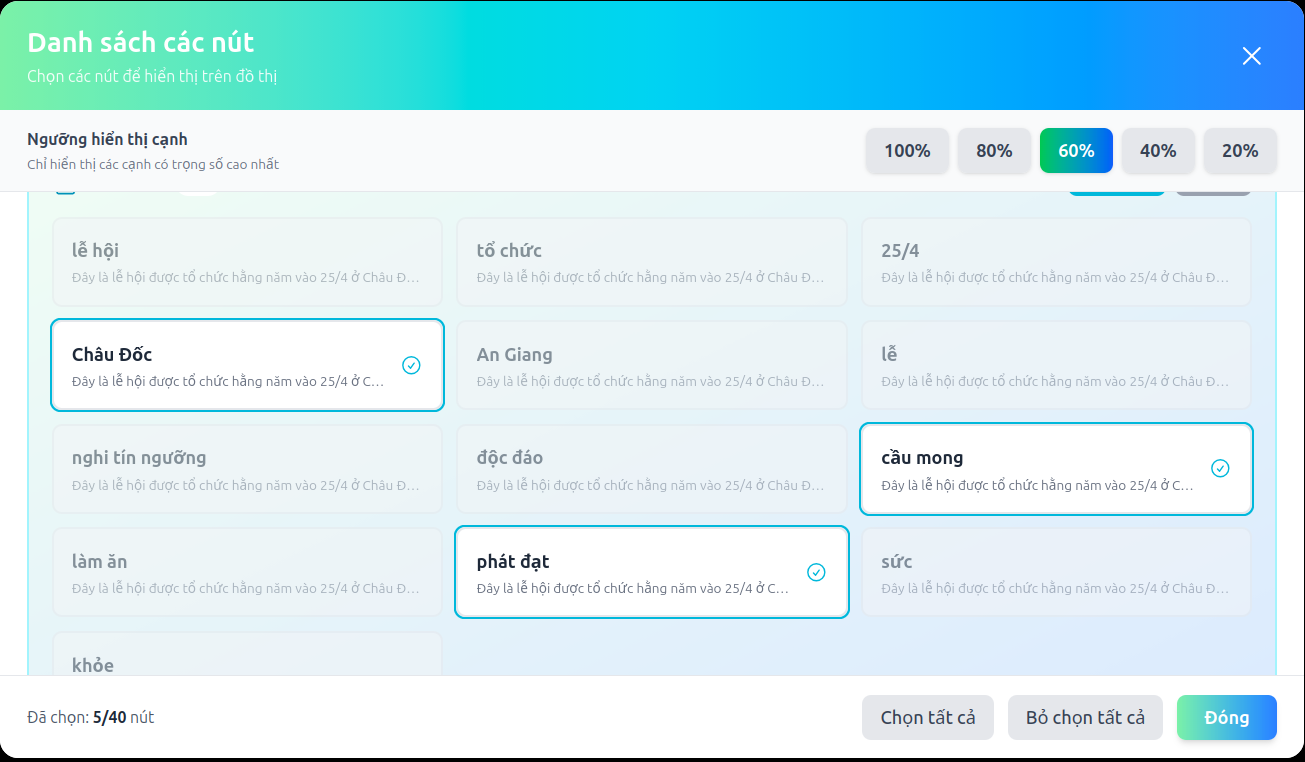
\includegraphics[width=0.9\linewidth]{images/part-02/chap-03/sec-01/DSNut-VanBan.png}}
    \vspace{0.1cm}
    \caption{Giao diện danh sách nút cho phương thức văn bản}
    \label{fig:/DSNut-VanBan}
\end{figure}

\newpage
\textbf{Danh sách nút âm thanh:} Khu vực này quản lý các nút đại diện cho đoạn âm thanh. Đặc biệt, hệ thống tích hợp trình phát media mini, cho phép người dùng nghe lại trực tiếp nội dung của đoạn âm thanh đó bằng cách nhấn vào biểu tượng phát.
\begin{figure}[H]
    \centering
    \fbox{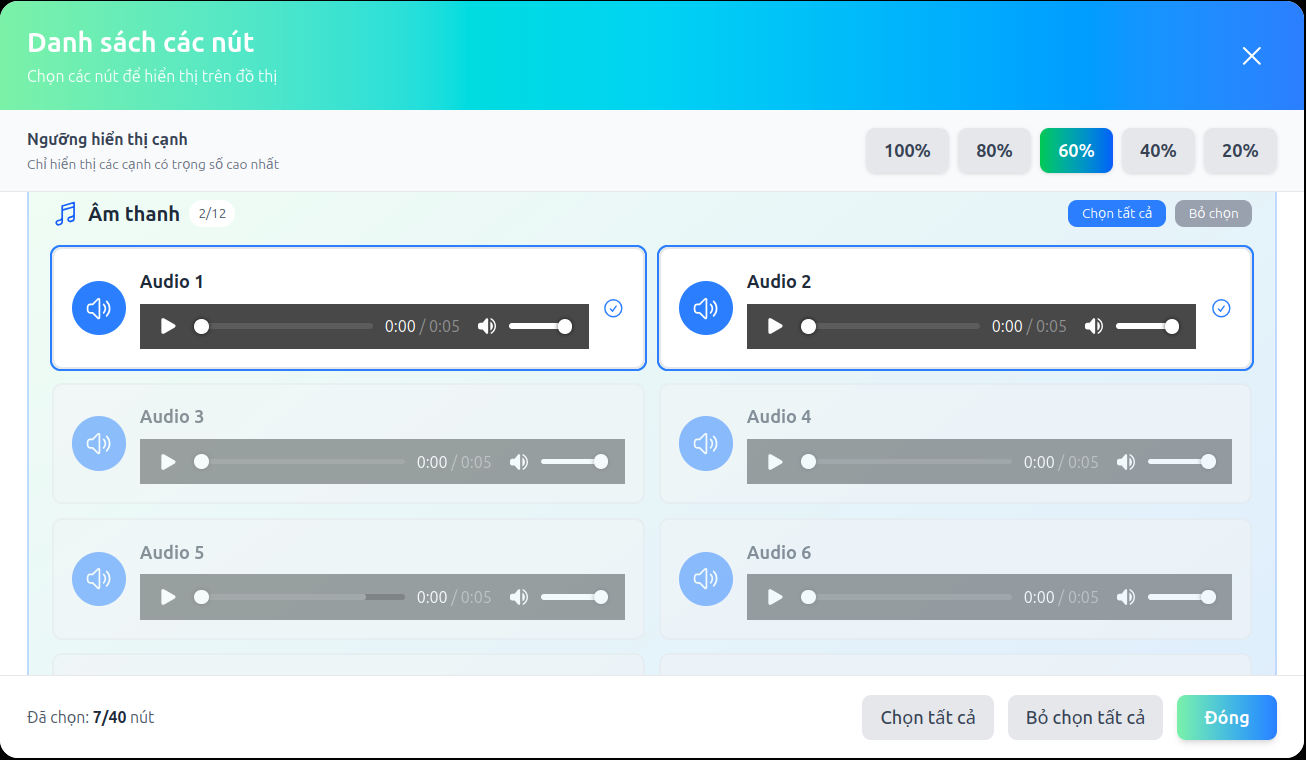
\includegraphics[width=0.9\linewidth]{images/part-02/chap-03/sec-01/DSNut-AmThanh.png}}
    \vspace{0.1cm}
    \caption{Giao diện danh sách nút cho phương thức âm thanh}
    \label{fig:DSNut-AmThanh}
\end{figure}

\textbf{Kết quả hiển thị đồ thị:} Hình minh họa dưới đây thể hiện cấu trúc đồ thị đa phương thức được trực quan hóa với bộ lọc 60\% trọng số cạnh cao nhất. Giao diện hỗ trợ tương tác toàn diện, cho phép người dùng phóng to, thu nhỏ và kéo thả các đỉnh để khám phá cấu trúc liên kết ngữ nghĩa giữa các phương thức.
\begin{figure}[H]
    \centering
    \fbox{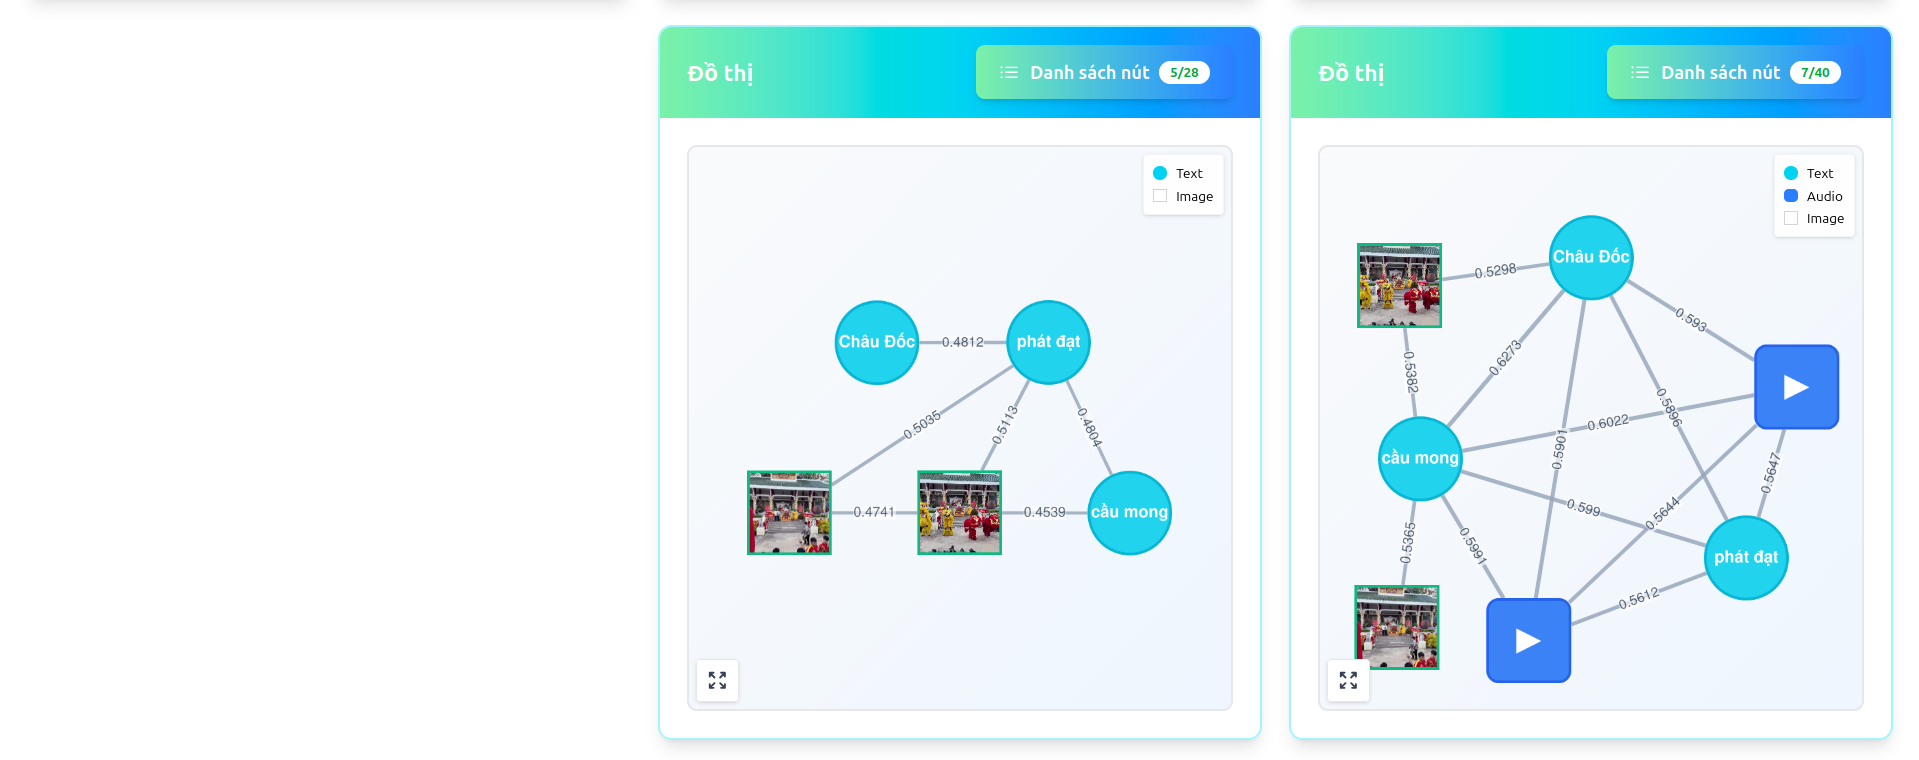
\includegraphics[width=0.9\linewidth]{images/part-02/chap-03/sec-01/KetQuaDoThi.png}}
    \vspace{0.1cm}
    \caption{\centering Giao diện hiển thị đồ thị tương tác}
    \label{fig:KetQuaDoThi}
\end{figure}